%----------------------------------------------------------------------------
\chapter{Evaluation}\label{sect:Comparison}\label{Ch6}
%----------------------------------------------------------------------------
%----------------------------------------------------------------------------
\section{Load testing results}
%----------------------------------------------------------------------------
%----------------------------------------------------------------------------
\subsection{Performance comparison}
%----------------------------------------------------------------------------
To examine the solution more in depth, I attempted to do a load test on the finished application. For this I used Azure Load Testing Preview (\cite{LoadtestOverview}). Setting up a test was pretty straightforward. I only had to create a testing resource and type in the test parameters as the test url, count of generated users and test duration to run a quick test (\cite{LoadtestQuickstart}). 

As I run more intense tests against my application, I pretty fast reached a point where the test stopped because of the high number of failed requests. Digging into the results file I found that after a point nearly all requests got the \emph{429 - Too Many Requests} response. I'm not entirely sure why has this happened but my guess is, that it was because I have a student Azure subscription and the amount of requests the static app can handle is limited down. Researching the issue I have found that for some users Azure Static Web Apps indeed caused similar problems.

So I decided to do a small test that fits into my resources and compare it to an SPA I created earlier and published to GitHub pages (\url{https://leventejuhos.github.io}). This is a one-page Angular app, it does not call any API. I tested both with 5 threads for 2 minutes.

I got the following test results for the two applications (see Figure \figref{swa} and Figure \figref{spa}):

\begin{figure}[!ht]
	\centering
	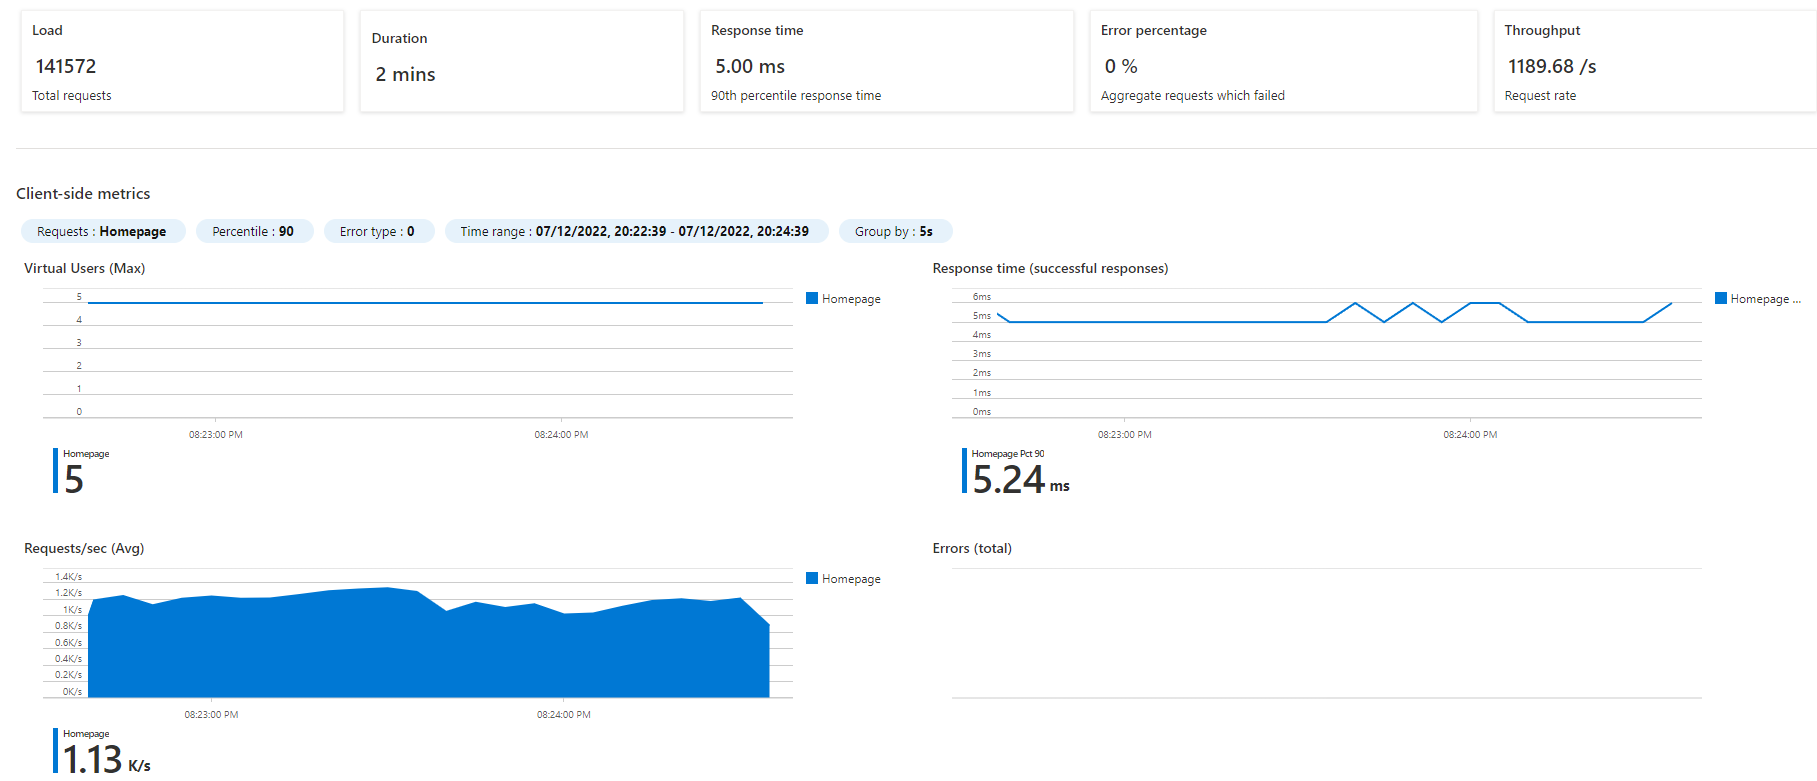
\includegraphics[width=150mm, keepaspectratio]{figures/loadtest/static_web_app.png}
	\caption{Static web app load testing results} 
	\label{fig:swa}
\end{figure}

\begin{figure}[!ht]
	\centering
	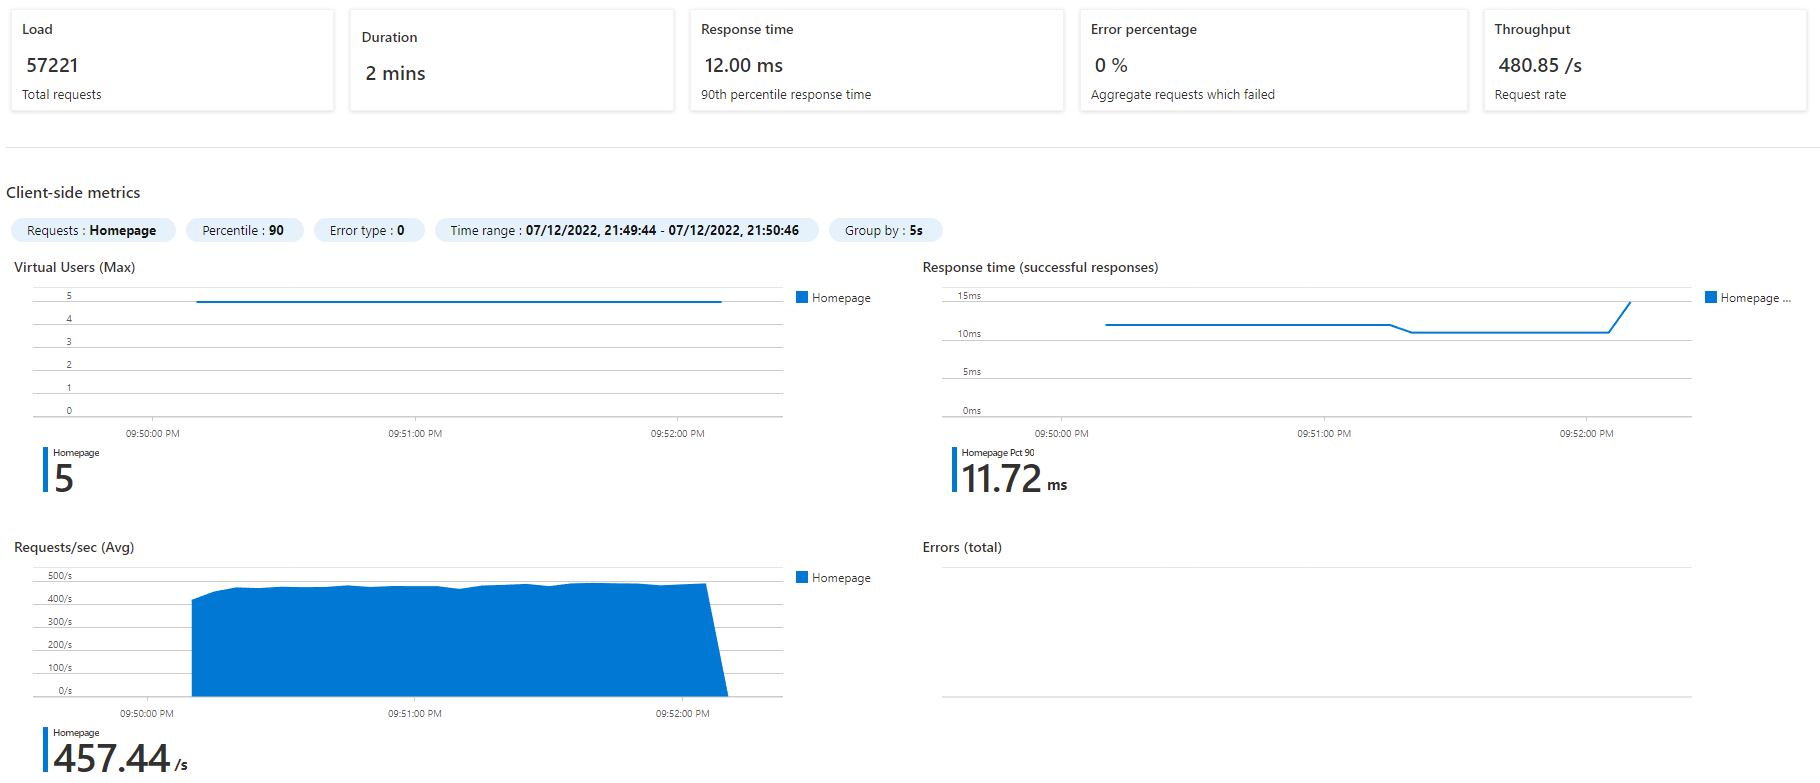
\includegraphics[width=150mm, keepaspectratio]{figures/loadtest/githubio-2.png}
	\caption{GitHub pages SPA load testing results} 
	\label{fig:spa}
\end{figure}

\begin{table}
	\begin{center}
		\begin{tabular}{||c c c c c c||} 
			\hline
			\makecell[c]{Name} & \makecell[c]{Thread count} & Duration  & \makecell[c]{Total requests} & \makecell[c]{Response time} & \makecell[c]{Requests/sec \\ (avg)}   \\ [0.5ex] 
			\hline\hline
			\makecell[c]{Azure \\ static web app} & 5 & 2 mins & 141572 & 5 ms & 1130/s \\
			\hline
			\makecell[c]{GitHub Pages \\ SPA} & 5 & 2 mins & 57221 & 12 ms & 457.44/s \\ [1ex] 
			\hline
		\end{tabular}
		\caption{App load testing results}
		\label{tab:AppLoadtest}
	\end{center}
\end{table}

When we compare the two (\tabref{AppLoadtest}) we see, that despite the Azure web app calls a function and gets a list of about 50 items, it does better than the other app without any database requests. The Azure app had a better response time, less than half of the SPA's and handled two and a half times the load volume of the SPA.

%----------------------------------------------------------------------------
\subsection{Service scalability}
%----------------------------------------------------------------------------

I gave another try to demonstrating the scalability of Azure by load testing one of the function apps. I set \url{https://restaurant-func-app-1.azurewebsites.net/api/getallrestaurants} function url as test url and run it for 2 minutes three times with different amount of virtual users.

\begin{table}
	\begin{center}
		\begin{tabular}{||c c c c c c||} 
			\hline
			\makecell[c]{Thread count} & Duration  & \makecell[c]{Total requests} & \makecell[c]{Response time} & \makecell[c]{Requests/sec \\ (avg)} & \makecell[c]{Error \\ percentage}  \\ [0.5ex] 
			\hline\hline
			10 & 2 mins & 14594 & 112 ms & 121.6/s & 0 \% \\
			\hline
			100 & 2 mins & 47244 & 364 ms & 377.46/s & 0 \% \\
			\hline
			250 & 2 mins & 60169 & 831 ms & 497.57/s & 0 \% \\ [1ex] 
			\hline
		\end{tabular}
		\caption{API load testing results}
		\label{tab:APILoadtest}
	\end{center}
\end{table}

This time none of the requests resulted in error. Comparing the results \tabref{APILoadtest} we notice, that although the average response time did increase along with the demand, the number of served request/sec also increased significantly. If we take a look at the response time diagram (\figref{APIlt}), it looks like the system adapted quickly to the growing demand. The response time dropped steeply during the first few seconds and maintained this level for the rest of the test. 

\begin{figure}[!ht]
	\centering
	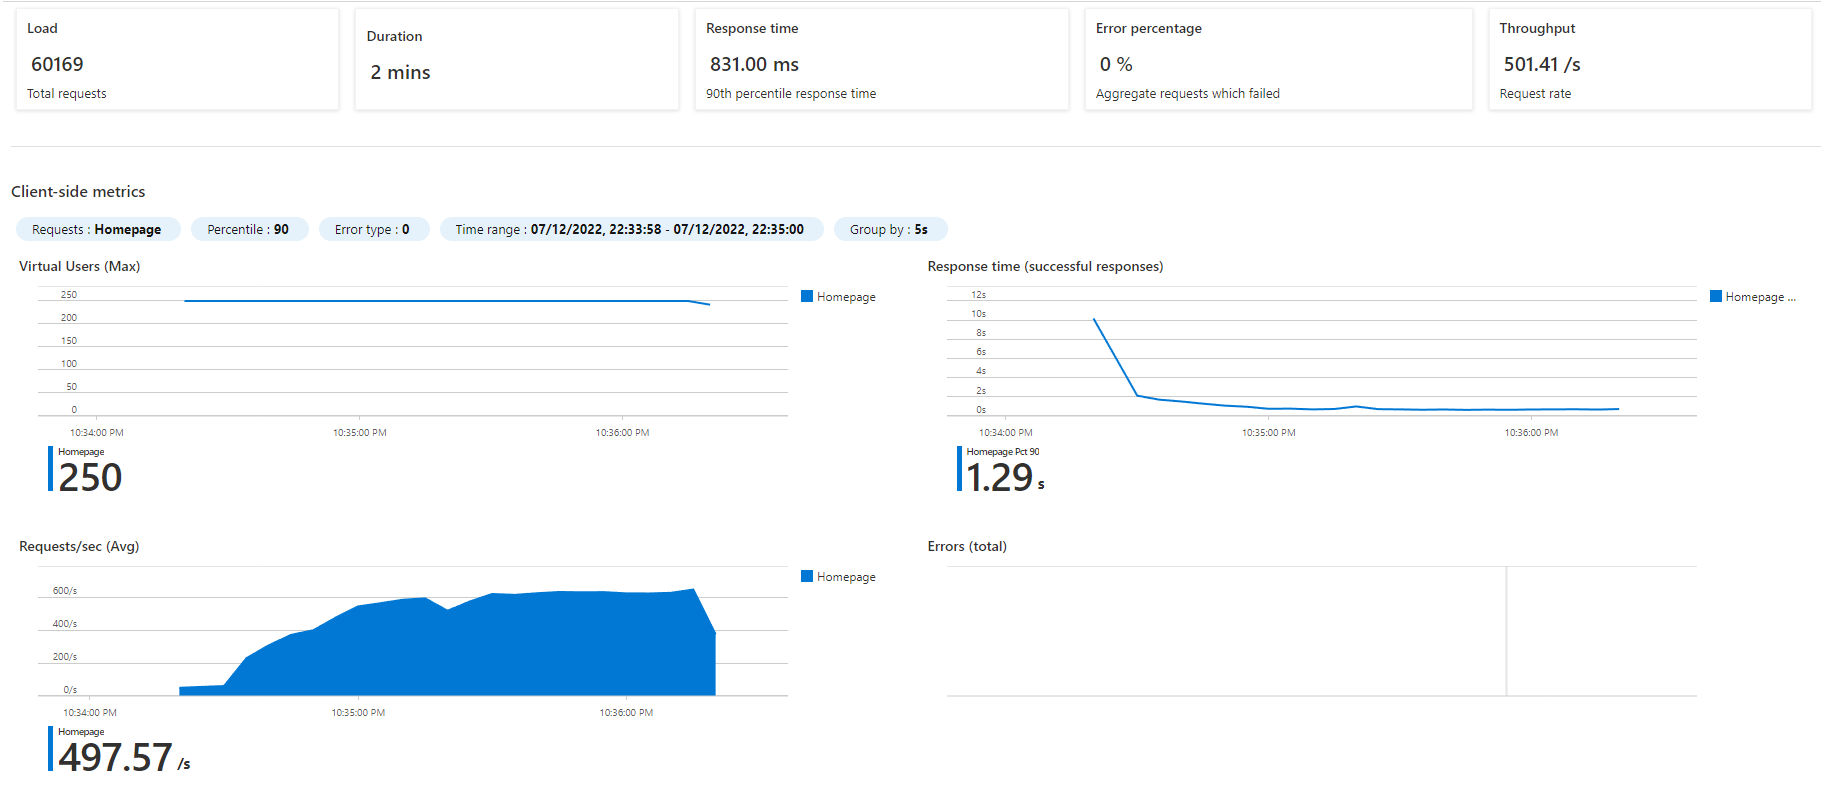
\includegraphics[width=150mm, keepaspectratio]{figures/loadtest/funcapp250-2.png}
	\caption{API load test with 250 threads} 
	\label{fig:APIlt}
\end{figure}

%----------------------------------------------------------------------------
\section{Solution complexity}
%----------------------------------------------------------------------------

On the frontend part there wasn't much difference between a conventional and an Azure serverless solution nor should be. Azure Functions, on the contrary, worked substantially differently than the solutions I used before. They required some extra maintenance in the Azure portal, but I found the functions' code to be more distinct and easier to test. Actually, I was surprised by how little code had to be written in order to communicate with the database in comparison with a conventional app. Overall, in my experience the reading and finding out how some components can be reached from the functions took much of the time not the actual coding.

%----------------------------------------------------------------------------
\section{Code portability}
%----------------------------------------------------------------------------

One drawback of the serverless approach is that the user have to choose one provider and the migration between them is not obvious. The Angular SPA is easily moved and can be published on any chosen platform. I could publish this exact same code anywhere else than Azure Static Web Apps without further modification. Unfortunately, we can't state the same about Azure Functions. Migrating a simple HTTP triggered function between cloud providers shouldn't be a huge hurdle. However, when Cosmos DB or other Azure specific components come into play then these have to be replaced by the other provider's solution, which will mean modifications in the function code as well. This is equally true to the data storage. As Azure is around for some time now there are solutions for moving data to other providers, but these will require extra steps from the developers' part (see an example here: \cite{MongoMoveData}).